\documentclass{IEEEtran}
\pagenumbering{gobble}

\usepackage[english]{babel}
\usepackage{amsmath}
\usepackage{bm}
\usepackage{listings}
\usepackage{blindtext}
\usepackage{multirow}
\usepackage{graphicx}
\usepackage{caption}
\graphicspath{ {./images/} }

\title{\textbf{NL2code}}

% Nischal Mahaveer Chand
% Varun Sundar Rabindranath
% Sai Krishna Karanan
\author{
    Sai Krishna Karanam 
    \texttt{karanam.s@husky.neu.edu}
    \and \\
    Nischal Mahaveer Chand 
    \texttt{mahaveerchand.n@husky.neu.edu}
    \and \\
    Varun Sundar Rabindranath 
    \texttt{rabindranath.v@husky.neu.edu}
}
\date{}

\begin{document}

    \maketitle

    \section{Introduction}
    \subsection{Importance of NL2code}
    Recent Integrated Development Environments (IDEs) provide a feature called ``context-aware 
    code completion'' which helps programmers speed up the coding process. This is very helpful for
    programmers who are already aware of the programming language syntax and the design paradigms.
    But, for beginners, this can be time consuming. \\
    \hspace*{4mm}The first step, for beginners, is to search how to implement the code in natural 
    language XXX. Due to the vast amount of resources available online, may unreliable or 
    outdated, having a local NL to code generator will make programming more enjoyable for 
    beginners and more productive for veteran programmers. And with the introduction of a new
    language almost everyday, it has become more and more important to establish an interface
    between NL and code. \\
    \hspace*{4mm}We aim to create neural based models to generate NL to code. Below we describe
    various attempts of implemening various encoder-decoder models for the same. It should be 
    noted that the project does not aim at providing a framework to build industry standard 
    deployable code, but is rather a proof-of-concept. The scope of this project is limited to 
    generate an accurate single line program statement given user intent in the form of a comment 
    or description. XXX \\

    \begin{tabular}{c l}
      \multicolumn{2}{ c }{Examples} \\
      \hline
      input & call the function sorted with argument x \\ 
      ref. & sorted(x) \\
      \hline
      input & for every k in keys \\
      ref. & for k in keys: \\
      \hline
    \end{tabular}

    \section{Related Word}
    Techniques to generate regular expressions [1], input parsers
    [2], UML diagrams, object oriented class layout, and general
    purpose code from Natural Language (NL) specification have
    been researched for a long time.

    Recent approaches in converting NL to executable source
    code predominantly use neural network techniques. These approaches follow two basic patterns. 
    One, is to directly convert
    NL to source code by modeling the task as a Sequence-to-Sequence conversion task, 
    using Recurrent Neural Networks
    (RNN) (Lili Mou et al., 2015, Ling et al., 2016) [3], [6] to that end.
    The other is to generate Abstract Syntax Trees (ASTs) from NL input, the deterministically
    convert the produced AST to code (Pengcheng Yin et al., 2017) [4].

    However, research [4] shows that the second approach is better
    than the first and emphasizes the use of syntax information of
    the target language, in NL to code tasks.
    We consider the recent research paper by Pengchen Yin
    et. al. [4] , on syntactic neural model for code generation
    as the primary motivation for this project. [4] proposes an
    approach where they translate NL to an Abstract Syntax Tree
    (AST) first, thus using the grammar of the target language
    as a prior knowledge. They report a 10\% absolute improvement in accuracy compared to 
    the previous state-of-the-art
    on standard datasets. Since, converting from AST to code
    can be done deterministically, their system always produces
    syntactically correct, executable code. This aspect is lacking
    in the Sequence-to-Sequence models, where the correctness of
    the generated code is not guaranteed. They use a Bidirectional
    LSTM (BiLSTM) network for encoding each word of the NL input as
    a context specific embedding, and an RNN as a decoder to
    generate an output AST.

    Maxim Robinovich et. al. [5], propose an approach similar
    to [4] for converting NL to AST. They confirm the experimental results of [4], thus again 
    emphasizing the use of target
    language syntax. However Maxim Robinovich et. al., have
    evaluated their system on a wider range of datasets achieving
    near state-of-the-art results on average.

    Pengcheg Yin et.al [4], report that 25\% of the errors incurred
    by their system, on one of the datasets, is due to the generated
    code only partially implementing the required functionality.
    We hypothesize that this could be due to the standard datasets
    used for this task being noisy. We propose a denoising procedure,
    explained in the Data Preprocessing section XXX to clean the dataset,
    thereby making the datasets more generic.

    Barone et. al, 2017, [7], hereafter referred to as the "Edinburgh paper",
    explores the difficulty of the code generation task and critiques
    the currently available datasets for this task. They also comment that
    the effectiveness reported by [4] should not be taken at face value.

    In the Edinburgh paper, Barone et al. scraped online Opensource Python
    repositories to extract ``docstring-code'' pairs. They propose that
    such data accurately represents the query/code pairs found in
    production environment. They used a Neural Machine Translation
    approach to translate docstring to code and reported a baseline
    BLEU score of 10.24, While [4] reports a BLEU score of 84.5 on the
    Django dataset.

    We wanted to check how [4] performs on a similar dataset.
    We scraped query-code pairs from the same online Opensource Python repositories as [7].
    [4], on our scraped dataset reports a BLEU score of only 14.2 which reaffirms
    the [7]'s claim that the reported effectiveness of various
    models could not be taken at face value and that the task of code generation
    is more difficult than what is conceived by the community.
    Much of this misrepresentation could be attributed to the fact that the
    datasets currently available for this task is very limited and noisy.

    \section{Dataset}
      \subsection{Standard Datasets}
        There are 3 datasets that have been used by the research community for the task
        of code-generation from the comments/query.
        \subsubsection{Django}
        Django dataset is a collection of 18000 lines of python code from the Opensource
        web framework, Django. The 18000 code statements have been manually annotated
        with a Natural language description. As a result of manual annotations, all the
        annotations are artificially descriptive of the corresponding code. This is
        the main drawback of the dataset, as the manual annotations rarely reflects
        the comments that programmers write in production environment. This can be seen
        in the following example.

        \begin{lstlisting}[frame=single,basicstyle=\small]
comment:
  raise and exception InvalidCacheBackendError 
  with string "Could not find config for '\%s' 
  in settings.CACHES" as argument , replace ' 
  \%s ' with alias .

code:
  raise InvalidCacheBackendError ( "Could not 
  find config for '\%s' in settings.CACHES" \% 
  alias )
        \end{lstlisting}

        \subsubsection{HearthStone}
        HearthStone dataset is a collection of 600 Python class - description pairs
        that implement cards for the online multiplayer card game HearthStone.
        The class - description pairs used to train and test are very similar, in that
        the any model trained on this dataset would be able to generate only a
        single template of code, like the one presented in the example. We could not
        use this dataset as the scope of the dataset very narrow and far from the case
        in general production environment. 

        \begin{lstlisting}[frame=single,basicstyle=\scriptsize]
card details:
  name: ['D', 'i', 'r', 'e', ' ', 
        'W', 'o', 'l', 'f', ' ', 
        'A', 'l', 'p', 'h', 'a']
  cost: ['2']
  type: ['Minion']
  rarity: ['Common']
  race: ['Beast']
  class: ['Neutral']
  description: ['Adjacent', 'minions', 'have', 
        '+', '1', 'Attack', '.']
  health: ['2']
  attack: ['2']
  durability: ['-1']

correspoding code:
  class DireWolfAlpha(MinionCard):
    def __init__(self):
      super().__init__( "Dire Wolf Alpha", 2, 
        CHARACTER_CLASS.ALL, CARD_RARITY.COMMON, 
        minion_type=MINION_TYPE.BEAST)
    def create_minion(self, player):
      return Minion(2, 2, auras=[Aura(ChangeAttack(1), 
                          MinionSelector(Adjacent()))])
        \end{lstlisting}

        \subsubsection{Edinburgh}
        The Edinburgh dataset is a collection of 200k docstring-code pairs scraped
        from Opensource python repositories. The docstring-code pairs actually
        reflect the comments written in production environment. However, the docstring
        reflects what a particular entity (method, class, function etc.) represents
        rather than how it is implemented. For the task of generating source code,
        we need information on implemention logic thus making the dataset unusable
        for our task.

        \begin{lstlisting}[frame=single,basicstyle=\scriptsize]
comment:
  Process elementNode by svgReader.

code:
  def processSVGElementtext(elementNode, svgReader):
    if svgReader.yAxisPointingUpward:
      return
    fontFamily = getStyleValue('Gentium Basic Regular', 
        elementNode, 'font-family')
    fontSize = getRightStripAlphabetPercent(getStyleValue
        ('12.0', elementNode, 'font-size'))
    matrixSVG = getChainMatrixSVGIfNecessary(elementNode, 
        svgReader.yAxisPointingUpward)
    loopLayer = svgReader.getLoopLayer()
    translate = euclidean.getComplexDefaultByDictionaryKeys(
        complex(), elementNode.attributes, 'x', 'y')
    for textComplexLoop in getTextComplexLoops(fontFamily, 
      fontSize, elementNode.getTextContent(), 
      svgReader.yAxisPointingUpward):
      translatedLoop = []
      for textComplexPoint in textComplexLoop:
        translatedLoop.append(textComplexPoint + translate)
      loopLayer.loops.append(matrixSVG.
        getTransformedPath(translatedLoop))
        \end{lstlisting}

      \subsection{Our dataset}
        \subsubsection{Scrapped Dataset}
        We scraped several of the Opensource python repositories from github and
        collected 12.5k pairs of code-comments after preprocessing the data.
        We found that the code is very project specific and the descriptions are context specific.
        This dataset also had the same issue as the Edinburgh dataset as in the descriptions
        mainly focused on why a code is written rather than how it's written.
        \subsubsection{Processed Django}
        Among all the datasets explored, the Django dataset represents the problem
        of converting NL to source code more accurately. But, as mentioned above
        the Django dataset is very noise, hence we denoise it (techniques
        mentioned in data preprocessing) before using it.

				\smallskip

				\begin{center}
        \begin{tabular}{ l | r }
					\hline
          \multicolumn{2}{ c }{Dataset Statistics} \\
					\hline
          Maximum query/comment length & 133 \\
					Maximum code length          & 701 \\
					Average query/comment length & 16.0 \\
					Average code length          & 8.7 \\
					Vocabulary size - Query      & 2205 \\
					Vocabulary size - Code       & 814 \\
					\hline
        \end{tabular}
				\end{center}

    \section{Models}
    We describe four models, each is build upon Pengcheng's model, but encodes the input in a 
    different method. First we start by briefly describing Pengcheng's model.

      \subsection{Pengcheng's model}
      Pengcheng recognized that adding syntax information to the model would give better
      predictions results XXX. Their model follows an encoder-decoder architecture, and takes
      the raw comment as input and generates an AST of the corresponding 
      code as output. \\
      \hspace*{4mm}The encoder comprises of an embedding layer and a BiLSTM
      layer. It takes a comment as input, embeds each word in the comment to give token embeddings
      TE\textsubscript{t}, for each word $ t $ in the comment. Each TE\textsubscript{t} is 
      sequentially feed into the 
      BiLSTM layer, to produces a Query Embedding (QE) of 128 dimensions. QE is passed to the
      decoder module. \\
      \hspace*{4mm}The decoder uses an Recurrent Neural Network (RNN) to sequentially generate 
      each node of the AST. Each node maps to a timestep in the RNN decoding process and thus, 
      generating the AST can be interpreted as unrolling the RNN. The RNN also maintains an 
      internal state to track the generation process at each timestep. \\
      \hspace*{4mm}Pengcheng tackles the problem with a probabilistic grammar model of
      generating an AST $ y $ given NL description $ x $: $ p(y\vert x) $. The best possible AST 
      $ \hat{y} $ is given by:

      \begin{equation}
        \label{eq:pengcheng}
        \hat{y} = \operatorname*{arg\,max}_y p(y\vert x)
      \end{equation}

      $ \hat{y} $ is then deterministically converted to the corresponding Python code using
      \texttt{astor} XXX.

      \begin{figure}[h]
        \centering
        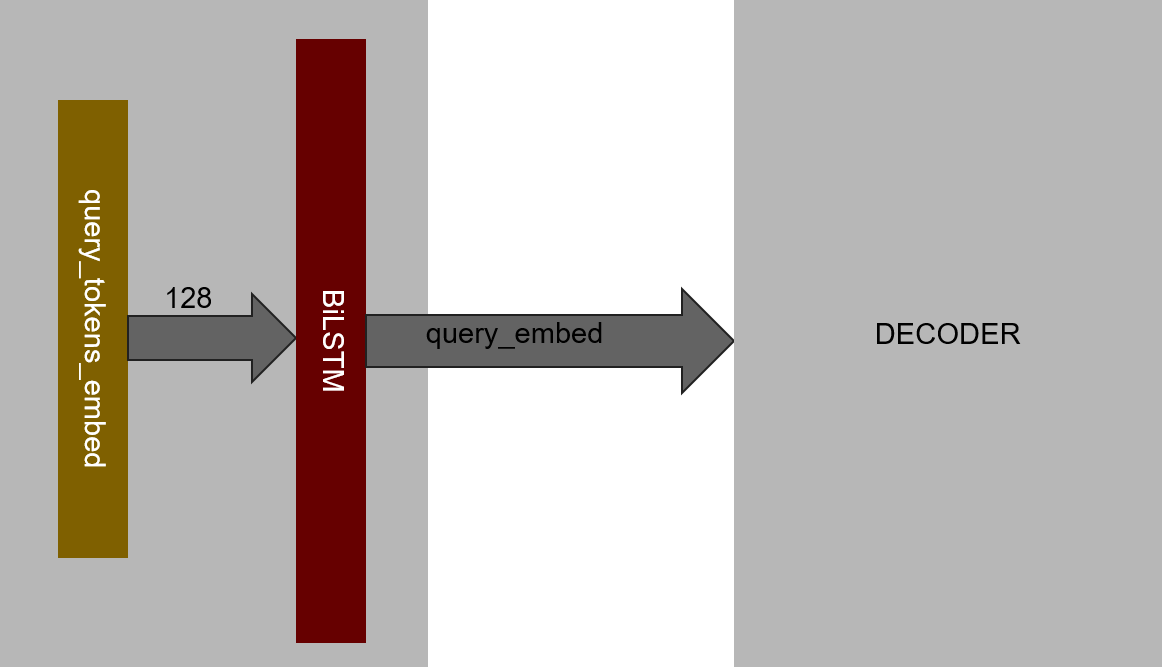
\includegraphics[width=8cm]{pengcheng.png}
        \caption{Architecture of Pengcheng's model. The encoder embeds each token of the NL input
        to give TE\textsubscript{t}, which is then passed into the BiLSTM layer. The encoder
        produces a 128 dimension QE which is feed into the decoder.}
        \label{fig:pengcheng}
      \end{figure}

      \subsection{Our models}
      As described, the decoder is already state-of-the-art XXX, and needs no further 
      modifications. All models described hereon use the same decoder architecture as Pengcheng's 
      model with modifications only to the encoder and the input data XXX. All models are 
      trained and tested using the dataset decribed in SECTION XXX. \\

        \subsubsection{Basic Concat (BC)}
        For our first attempt to incorporate syntax information into the encoder, we decided to 
        concatenate (shown as ``:'') the POS ID and phrase ID of each token to the corresponding 
        token embedding, giving the Augmented Token Embedding (ATE). The ATE is then feed into 
        a modified BiLSTM layer that takes 130 dimension embeddings, rather than the default 128 
        dimensions. \\

        \begin{figure}[h]
          \centering
          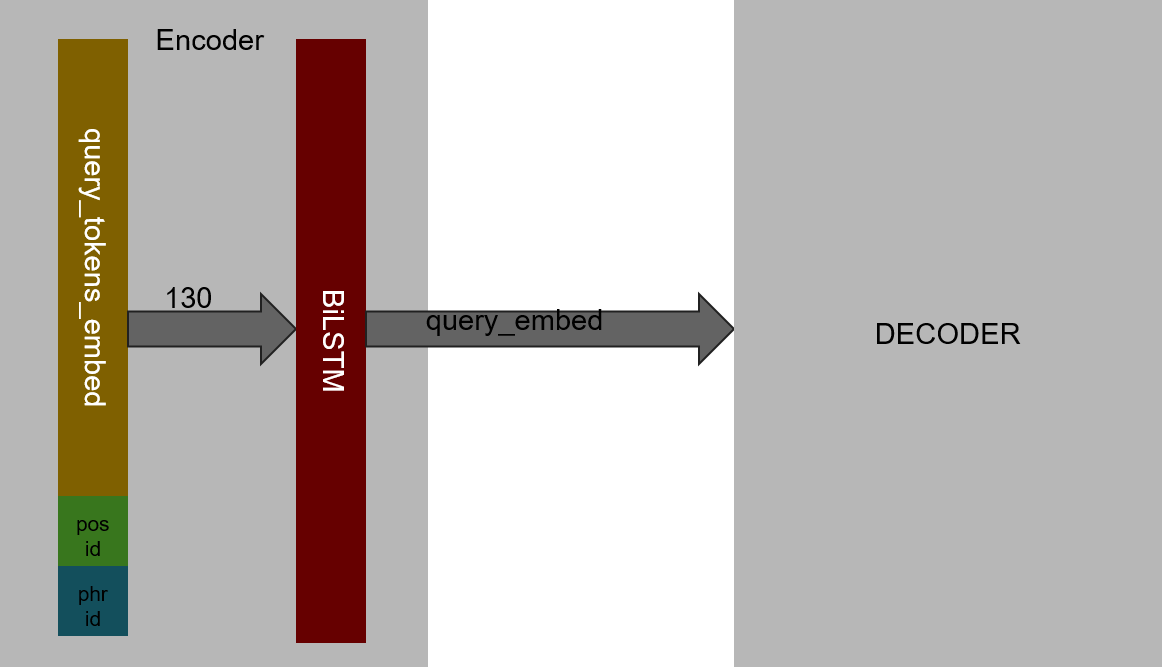
\includegraphics[width=8cm]{bc.png}
          \caption{Architecture of Basic Concat model. Notice that the POS ID and phrase ID
          are directly appended to the corresponding TE. The resulting 130 dimension embedding
          is passed to the BiLSTM.}
          \label{fig:bc}
        \end{figure}

        \hspace*{-3.5mm}TE\textsubscript{t} dimension: 128 \\
        POS\_ID\textsubscript{t} and Phrase\_ID\textsubscript{t} dimension: 1 each; total 2 \\
        ATE\textsubscript{t} dimension = 130 \\
        \hspace*{-3.5mm}ATE\textsubscript{t} = \lbrack TE\textsubscript{t} : 
        POS\_ID\textsubscript{t} : Phrase\_ID\textsubscript{t}\rbrack \\
        QE = BiLSTM(ATE) \\

        \subsubsection{Linear Projection (LP)}
        To add syntactic information over a sequence of tokens, we used an embedding layer for
        POS and phrase tags. The resulting TE, POS embedding (POSE), and Phrase embedding (PhE) are
        then concatenated to produce the ATE; which is a $ (128 * 3) $ dimension vector. We then
        apply a linear projection (using a dense layer with the linear activation function) to 
        give ATE Projected (ATEP) which is passed to BiLSTM. \\

        \begin{figure}[h]
          \centering
          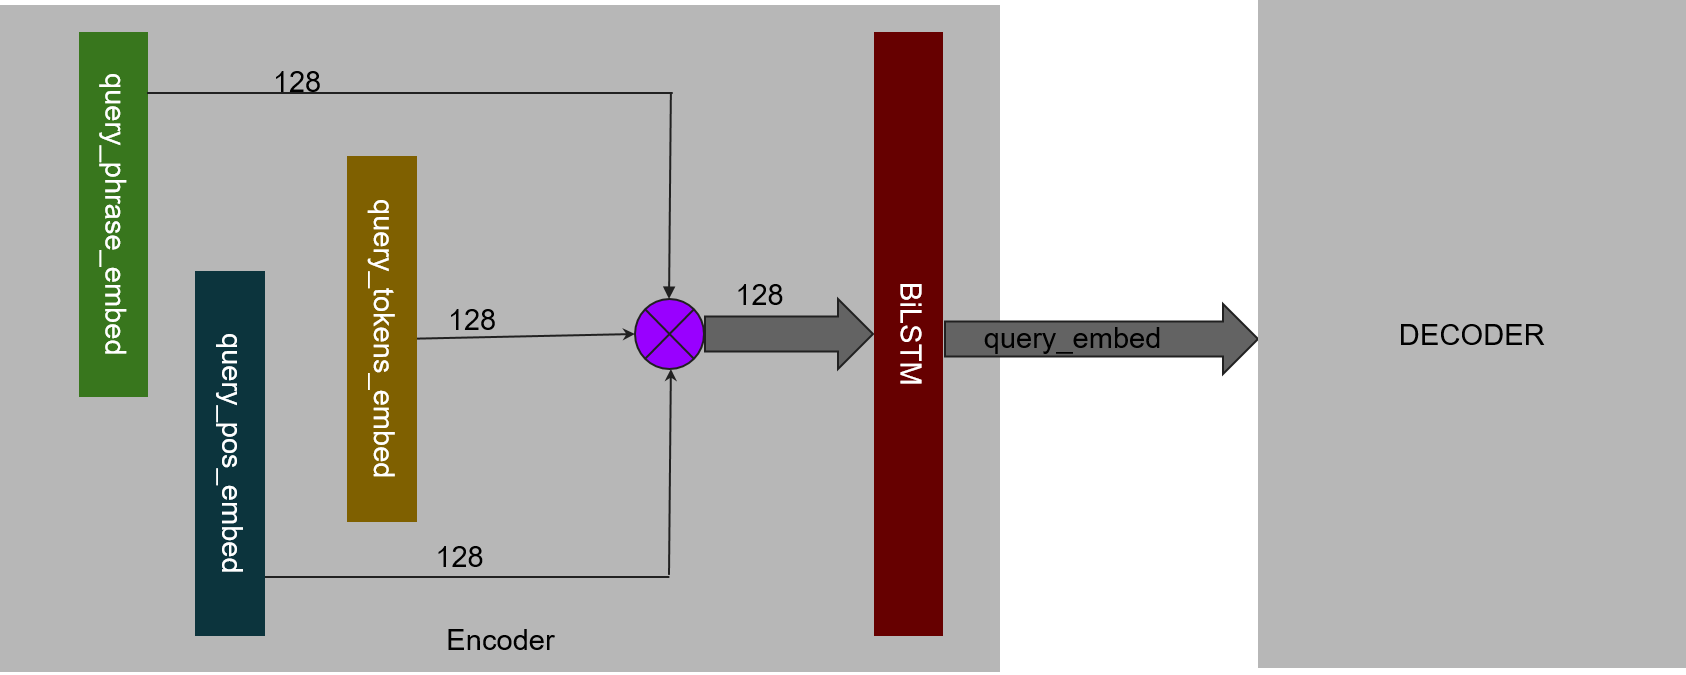
\includegraphics[width=8cm]{lp.png}
          \caption{Architecture of Linear Projection model. Each embedding - TE, POSE, and PhE 
          are concatenated and projected (shown as purple circles). The resulting ATEP is passed
          to the BiLSTM.}
          \label{fig:lp}
        \end{figure}

        \hspace*{-3.5mm}TE\textsubscript{t} dimension: 128 \\
        POSE\textsubscript{t} dimension: 128 \\
        PhE\textsubscript{t} dimension: 128 \\
        Dense = (128 * 3) input nodes, 128 output nodes \\ 

        \hspace*{-3.5mm}ATE\textsubscript{t} = [TE\textsubscript{t} : 
        POSE\textsubscript{t} : PhE\textsubscript{t}] \\
        ATEP\textsubscript{t} = Dense(ATE\textsubscript{t}) \\
        QE = BiLSTM(ATEP) \\

        \subsubsection{Linear Projection Reduced Dimension (LPrd)} 
        Subsequently, we noticed that the POS and Phrase vocabulary sizes were relatively smaller
        than token vocabulary size. To avoid redundancy XXX, we reduce the embedding dimensions
        of POSE and PhE to 8 and 32 respectively. The process described in LP is then repeated. \\

        \begin{figure}[h]
          \centering
          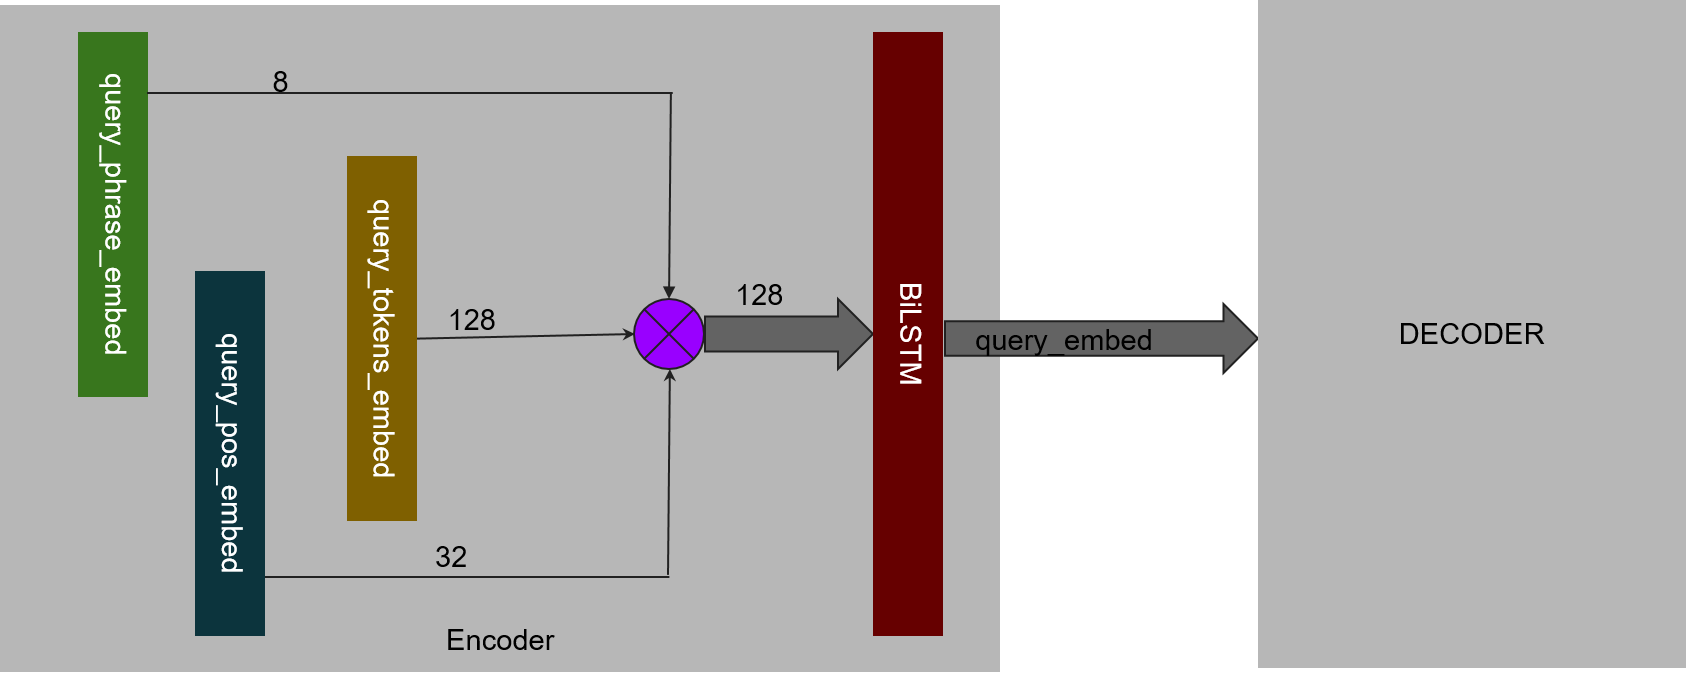
\includegraphics[width=8cm]{lprd.png}
          \caption{Architecture of Linear Projection Reduced Dimension model. Same as LP, but with
          reduced dimensions for POSE and PhE.}
          \label{fig:lprd}
        \end{figure}

        \hspace*{-3.5mm}TE\textsubscript{t} dimension: 128 \\
        POSE\textsubscript{t} dimension: 8 \\
        PhE\textsubscript{t} dimension: 32 \\
        Dense = (128 + 8 + 32) input nodes, 128 output nodes \\ 

        \hspace*{-3.5mm}ATE\textsubscript{t} = [TE\textsubscript{t} : 
        POSE\textsubscript{t} : PhE\textsubscript{t}] \\
        ATEP\textsubscript{t} = Dense(ATE\textsubscript{t}) \\
        QE = BiLSTM(ATEP) \\

        \subsubsection{Raw Query Independent Preprojection (AdvLP)}
        Rather than applying one linear projection on ATE, we apply two here, where the first is 
        independent of the input query. POSE and PhE are concatenated and projected to create
        Augmentation Embedding (AE), which is then concatenated with TE and projected to produce
        QE. We hypothesize that this would preserve most of the information from the input query
        during projection. \\

        \begin{figure}[h]
          \centering
          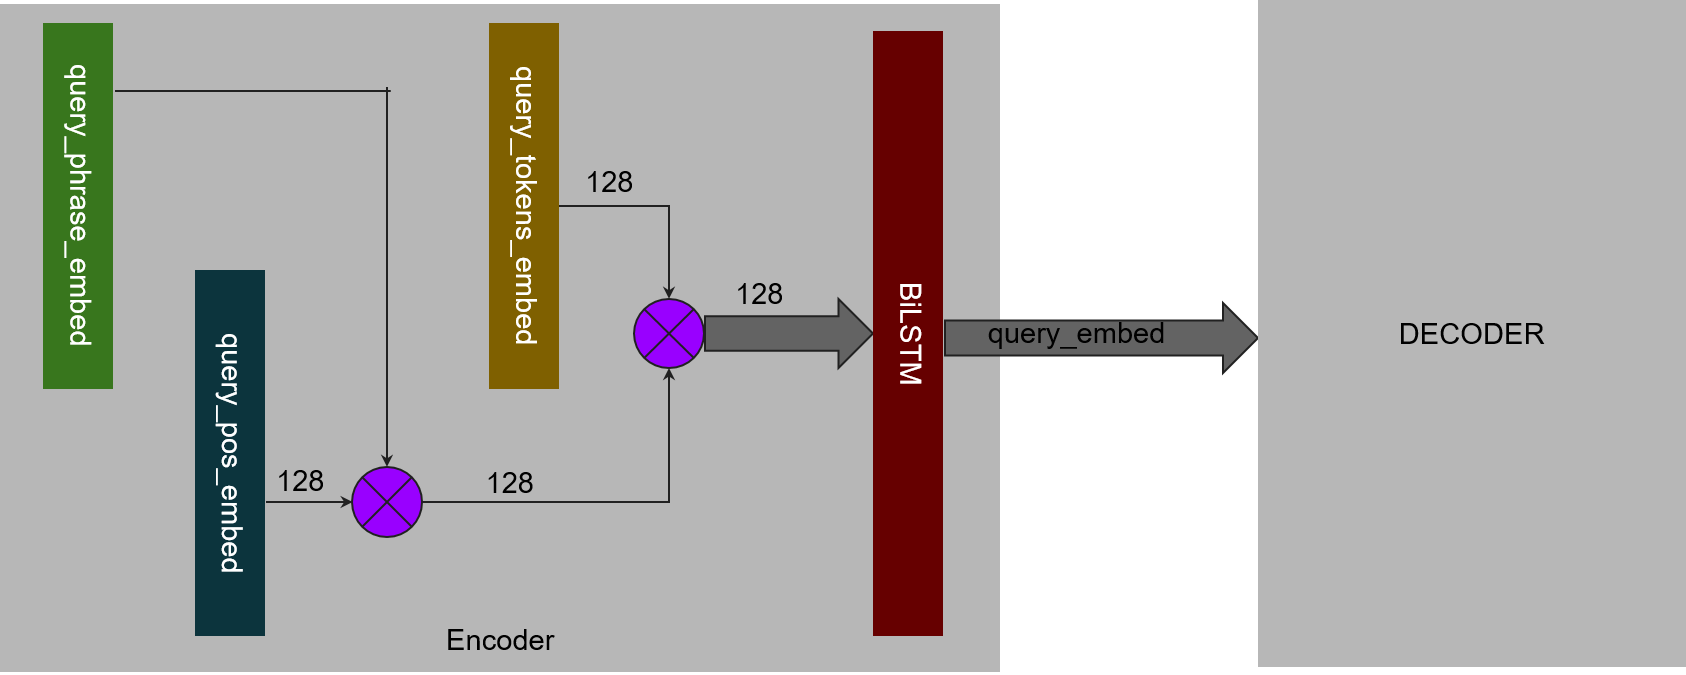
\includegraphics[width=8cm]{advlp.png}
          \caption{Architecture of Raw Query Independent Preprojection model. POSE and PhE are
          concatenated and projected independent of the input query. The resulting is 
          concatenated with TE and projected to produce QE.}
          \label{fig:advlp}
        \end{figure}

        \hspace*{-3.5mm}TE\textsubscript{t} dimension: 128 \\
        POSE\textsubscript{t} dimension: 128 \\
        PhE\textsubscript{t} dimension: 128 \\
        Dense = (128 * 2) input nodes, 128 output nodes \\ 

        \hspace*{-3.5mm}AE\textsubscript{t} = Dense([POSE\textsubscript{t} : 
        PhE\textsubscript{t}]) \\
        ATE\textsubscript{t} = [TE\textsubscript{t} : AE\textsubscript{t}] \\
        ATEP\textsubscript{t} = Dense(ATE\textsubscript{t}) \\
        QE = BiLSTM(ATEP) \\

      % end of Models

    \section{Experiments}
    All decoder dimensions and configurations are left untouched and are thus the same as in
    Pengcheng's model. For each of the above models, the embedding sizes are as described Models.
    Each model is run for a maximum of 50 epochs, with early stopping if the validation
    metrics do not change for 10 epochs.

    \section{Results}
    We evaluate our model on two metrics: BLEU and Accuracy.
    \begin{enumerate}
      \item BLEU: NLTK's \texttt{bleu\_score} function is used with NIST geometric sequence 
        smoothing.
      \item Accuracy: We use exact match for accuracy. +1 if the token matches the reference 
        exactly, 0 otherwise. The total is normalized by the number of the prediction. \\
    \end{enumerate}
    \begin{center}
    \resizebox{8cm}{!} {
      \begin{tabular}{ c | c || c | c }
        \hline
        \multicolumn{2}{ c ||}{\multirow{2}{*}{Models}} & \multicolumn{2}{ c }{Metrics} \\
        \cline{3-4}
        \multicolumn{2}{ c ||}{} & BLEU & Accu. \\
        \hline
				\hline
        \multicolumn{2}{ c ||}{Pengcheng} & 84.5 & 71.6 \\
        \multicolumn{2}{ c ||}{Base} & 73.2 & 67.9 \\
        \hline
        \multirow{4}{*}{NL2code} & BC & 73.6 & 69.4 \\
        & LP & \underline{74.3} & \underline{69.7} \\
        & LPrd & 73.6 & 69.0 \\
        & AdvLP & 73.7 & 69.1 \\
        \hline  
      \end{tabular} }
    \end{center}

    \section{Conclusion}
    \blindtext

    % \bibliographystyle{ieeetran}
    % \bibliography{report}

\end{document}
